\documentclass[conference]{IEEEtran}
\usepackage{graphicx}
\usepackage{amsmath}
\usepackage{cite}
\usepackage{subcaption} % For subfigures and captions
\usepackage{caption}
\captionsetup[figure]{labelformat=simple, labelsep=period}


\title{Crop Row Detection and Waypoint Definition Using Aerial Images of Fields}

\author{
    \IEEEauthorblockN{Alireza Amiri}
    \IEEEauthorblockA{Department of  Mechatronics Engineering\\
    K N. Toosi University of Technology\\
    Tehran, Iran\\
    ali.amiri@email.kntu.ac.ir}
    \and
    \IEEEauthorblockN{Saeed Khankalantary}
    \IEEEauthorblockA{Department of Mechatronics Engineering\\
    K N. Toosi University of Technology\\
    Tehran, Iran\\
    s.kalantary@kntu.ac.ir}
}

\begin{document}

\maketitle

\begin{abstract}
As autonomous agriculture evolves, using wheeled mobile robots for various tasks necessitates precise waypoint generation to accurately define the robots' paths. This paper introduces a method that leverages aerial imagery to detect crop positions and determine waypoints. A specialized hardware setup, consisting of a high-resolution camera, wireless transmitter, and receiver, is developed to capture and transmit live images of the agricultural field. In the image processing stage, crops are identified through two parallel techniques—Unet and K-means clustering. Subsequently, the Hough Transform is applied to detect crop row lines, refined through filtering to ensure that a single, accurate line represents each row. Finally, by selecting specific points on the paths between these rows and converting them into global coordinates, the system facilitates real-time crop detection and precise waypoint generation, supporting autonomous navigation for agricultural robots.
\end{abstract}

\begin{IEEEkeywords}
Crop Row Detection, Hough Transform, Image Processing
\end{IEEEkeywords}

\section{Introduction}
The integration of advanced technologies, such as artificial intelligence, sensing systems, and autonomous robots, is crucial in addressing global food challenges by enhancing agricultural productivity and sustainability \cite{b2,b3}. Precision Agriculture (PA) has emerged as a smart management system that optimizes input distribution, such as water and fertilizers, based on site-specific needs, thereby improving crop yield and resource-use efficiency while minimizing environmental impact \cite{b5,b6}. 
Mobile robots in precision agriculture have been utilized in various field tasks, such as fertilization, irrigation, weeding, harvesting, and crop picking \cite{b2,b3}.

In precision agriculture, traditional GPS-based path planning for agricultural machinery remains common, yet it presents challenges, such as the risk of seedling injury due to deviations between the ideal path and the actual crop rows \cite{b1}. To address these issues, the use of machine vision-based crop row detection on unmanned agricultural machinery has gained attention, allowing for real-time, precise path planning that minimizes crop damage \cite{b1,b8}. However, the unstructured agricultural environment complicates accurate navigation and autonomous operations, necessitating the integration of onboard sensors, such as scanning lasers and machine vision cameras, to enhance the robot's ability to sense and interact with its surroundings \cite{b2,b3}. Despite these advancements, ground-based platforms face challenges, including soil compaction and vibrations from uneven terrain, which can be mitigated by utilizing UAVs for high-resolution, low-altitude aerial sensing \cite{b10}.

Unmanned Aerial Vehicles (UAVs) have increasingly become a vital tool in precision agriculture, offering a flexible, cost-effective platform for high-resolution remote sensing  \cite{b9,b12}. UAVs can capture detailed imagery under different conditions, providing fine spatial resolutions and covering significant areas, which is essential for monitoring crop variability and supporting temporal analysis \cite{b10,b12}. These platforms excel in applications such as vegetation segmentation, weed management, and crop row detection, filling the gap between terrestrial and satellite-based remote sensing \cite{b7,b13}. Despite certain limitations, such as flight endurance, the ability to conduct self-automated flights and provide timely data collection makes UAVs an indispensable tool in modern agriculture \cite{b11,b13}. However, aerial image post-processing is necessary to differentiate crop rows from soil and weeds, highlighting the complexity of their integration in precision farming \cite{b6}.
The initial step in the procedure of crop row detection is semantic segmentation of aerial images, to determine the positions where vegetation exists. Different approaches were experimented in previous works in order to achieve a trusted and accurate model for segmentation. 


The literature on crop row detection encompasses a range of approaches, each employing distinct methodologies to enhance precision in agricultural applications. Vegetation indices (VIs) like NDVI, ExG, and SAVI are frequently utilized as inputs for various detection methods, including thresholding algorithms, K-means clustering, and the Minimum Distance to the Mean (MDM) classifier. These methods are instrumental in segmenting vegetation from soil backgrounds and effectively identifying crop rows \cite{b1,b6,b13}. Fusion approaches, which combine RGB and NDVI data, are also explored to improve segmentation processes, particularly for autonomous robotic navigation in agricultural fields \cite{b5}.

AI-based approaches have gained prominence, particularly deep learning models, which have significantly improved detection accuracy. For instance, CRowNet, which combines a convolutional neural network (CNN) with the Hough transform, demonstrates robust detection capabilities across various crop types and field conditions, achieving high detection rates even in complex scenarios like curved or intersecting rows \cite{b8,b14}. Additionally, networks like U-Net, SegNet, and ModSegNet are used in conjunction with both traditional and deep learning-based semantic segmentation methods. These networks have shown varying degrees of effectiveness, with deep learning models generally outperforming classical approaches, particularly in challenging conditions where traditional methods may falter \cite{b5,b13}.

Traditional computer vision techniques are widely employed in crop row detection, with the Hough Transform being a prevalent method for line detection \cite{b2,b15}. Despite its extensive use, the Hough Transform has inherent limitations such as high computational complexity and sensitivity to noise, which compromise its suitability for real-time applications \cite{b2}. To address these issues, various adaptations, including the Probabilistic and Multi-scale Hough Transforms, have been developed \cite{b2}. Moreover, combining the Hough Transform with deep learning has shown to improve detection accuracy \cite{b8}. Linear Regression is another commonly used technique, valued for its simplicity and computational efficiency, especially when integrated with preprocessing steps like image segmentation and feature extraction \cite{b2,b3}. Other methods such as the Horizontal Strips Method and Blob Analysis are also utilized in crop row detection. The Horizontal Strips Method enhances computational efficiency by bypassing additional segmentation steps but may suffer from accuracy issues due to factors like camera angle and missing rows \cite{b2}. Blob Analysis, which groups connected pixels into blobs to generate crop rows, can struggle in environments with high weed density \cite{b2}. The Random Sample Consensus algorithm is another approach, providing robust row detection by estimating mathematical models from data with outliers, though its effectiveness depends on factors such as the quality of extracted feature points \cite{b2}. Machine learning methods, including clustering techniques like K-means and deep learning models such as Faster R-CNN, YOLOv3, and SegNet, are increasingly being applied in this domain \cite{b2,b5}. These methods offer significant advantages, although challenges remain, particularly in handling varying field conditions and limited annotated data \cite{b2,b5}.

In precision agriculture, extracted crop row and inter-row information serves as a foundation for various tasks, such as guiding autonomous ground vehicles by defining navigation paths between rows, which are crucial for tasks like automatic path computation and the development of vigor maps for field partitioning \cite{b11}. For aerial images, the navigation path is identified as the line between two crop rows, while for unmanned agricultural vehicles, it is defined by the central angle between two rows\cite{b1}.

This paper is structured as follows. In Section 
\ref{Data Acquisition}
, the hardware setup for aerial imagery data acquisition is detailed. Section
\ref{Image Processing}
explains the image processing procedure, including image splitting and the application of two methods—K-means clustering and the U-Net model—for detecting plants from aerial images. Section
\ref{Crop Row Detection}
describes the crop row detection process, utilizing both linear regression and the Hough transform. Section D outlines the path detection process. In Section E, the reconstruction of the split images is addressed. Finally, Section F explains the conversion of local waypoint positions in the images to global coordinates.

\begin{figure}[htbp]
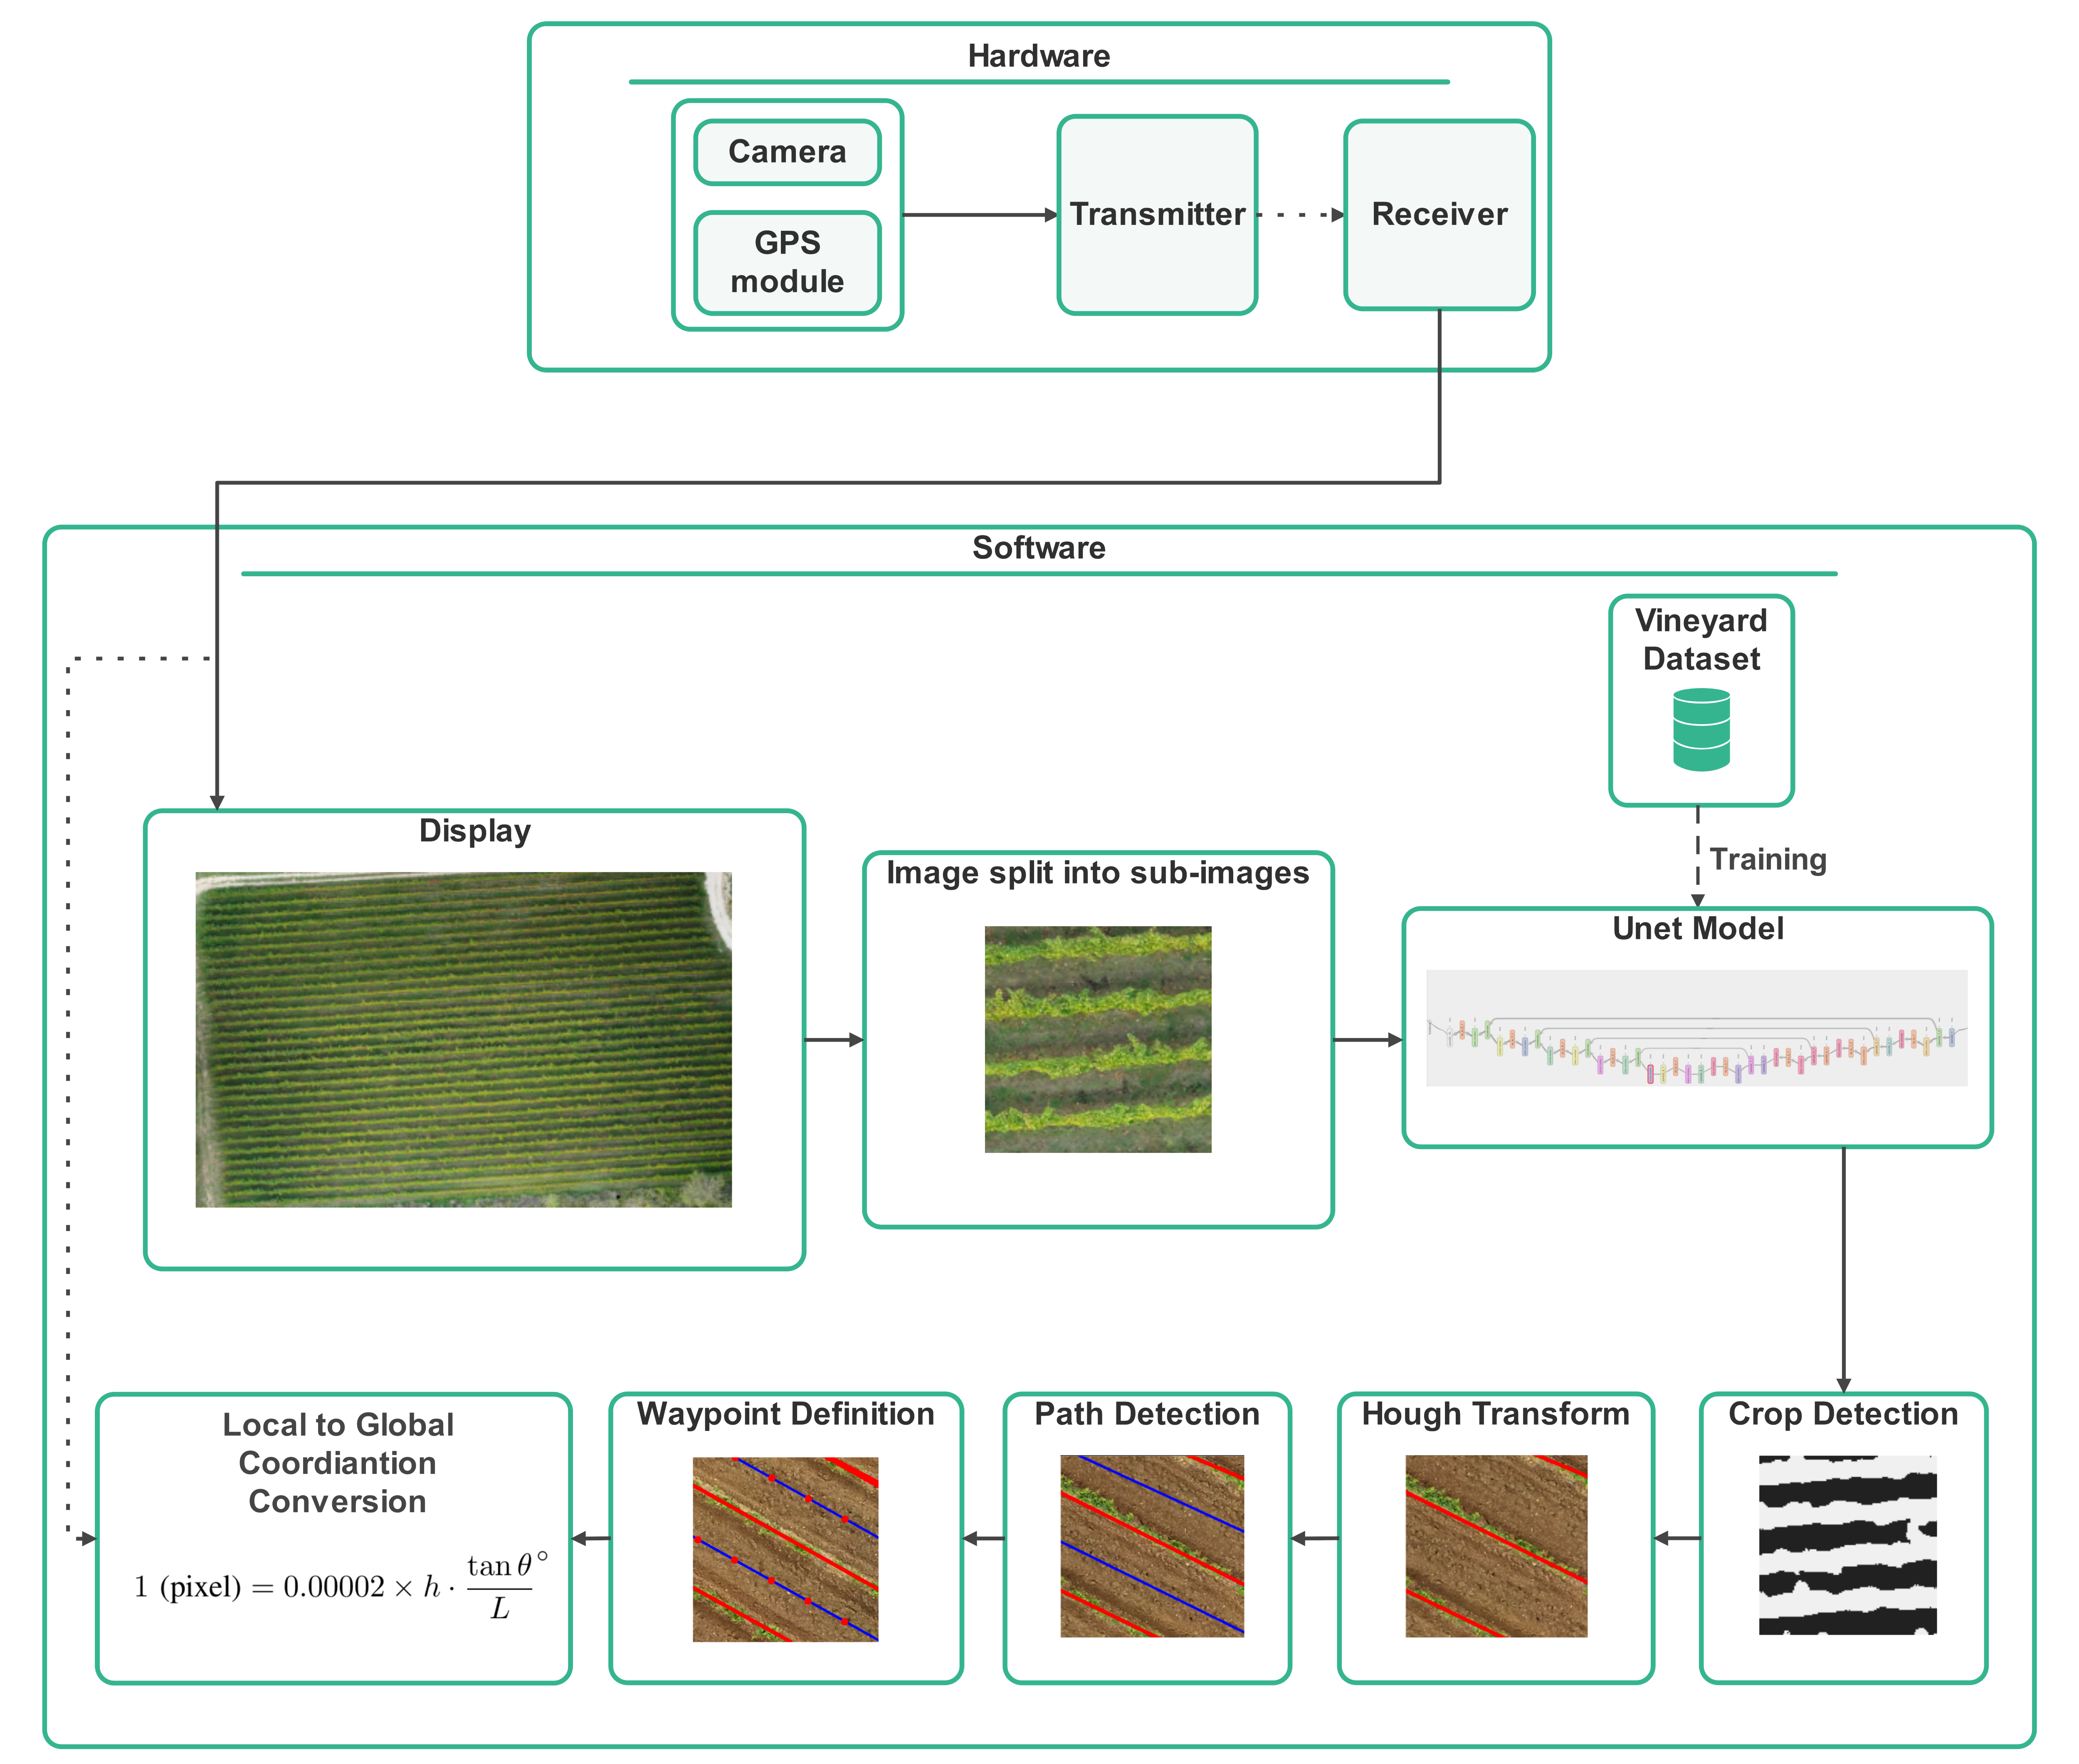
\includegraphics[width=\linewidth]{Block Diagram.png}
\caption{Pipeline of waypoint detection using aerial images}
\label{fig1}
\end{figure}

\section{Data Acquisition}\label{Data Acquisition}
In response to the need for live waypoint generation in agricultural fields, a hardware setup is required to provide the necessary environmental information. This system has the role of capturing and transmitting data to the software unit, where the processing will take place. In the context of this project, a lightweight camera is crucial to take high-resolution aerial images of the target field which will be the main data source for the image processing algorithm. Several cameras including Sequoia 
\cite{b9,b4,b7,b6}
, Micasense RedEdge
\cite{b9,b14}, and DJI Zenmuse X7
\cite{b5} were utilized in similar projects. Considering the specifications of these cameras and crop row detection algorithms developed based on their aerial images, it was concluded that having high-resolution RGB images meets the needs of this project. Although NIR band contains valuable information about the field and can be used for vegetation segmentation, they are too sensitive to environmental conditions such as temperature and might lead to the poor performance of the software
\cite{b5}. In conclusion, the Gopro HERO4 camera was acquired for this project. The specifications of this camera including its light weight, high-quality RGB images, and durability make it a suitable choice for aerial imagery. 
Besides the camera, a radio transmission system consisting of power supplies, a transmitter, and a receiver was developed to provide live data transfer between the mounted camera on the UAV and the computer with an image processing program. 
Also, the last step of this project, which is the conversion of pixel coordination on the images to global coordination, requires the global coordination of the camera at the time of photo capturing as a reference. A Ublox-Neo-6m GPS module must be mounted on the camera UAV to provide this information.
NEED AN IMAGE OF GOPRO


\section{Image Processing}\label{Image Processing}
The main contribution of this paper lies within this section, to develop an image-processing pipeline to determine the position of pixels which are located in the path between the crops. The Figure shows the procedure proposed in this paper. Initially, the aerial images captured with the camera are split into sub-images, and then during a semantic segmentation process, a binary mask is generated for each sub-image showing the positions of vegetation and background. In the next step, using Hough Transform, crop rows are detected. After defining the path line, a desired number of equally spaced points are selected on this line, and their position is recorded for later steps. Finally, the sub-images and their local waypoint coordinates are reconstructed and form the original input image.



\subsection{Preprocessing}\label{Preprocessing}
High-resolution aerial images covering large areas are typically too large to be used directly in image processing algorithms and networks. Besides, due to the variation in terrain topologies, the non-uniform shape of crop rows -including curved or irregular shapes- is common in some agricultural fields
\cite{b2, b3, b14}.
Given this information, the calculation of a straight line for an entire crop row in the original image is not an accurate approach for crop row detection.
To address this issue, the aerial image is initially split into equal-sized sections with a static image size of 512*512 pixels. These sub-images are named accordingly to be reconstructed after the image-processing procedure is finished. their chosen size ensures compatibility with the algorithms and networks designed in the later steps of the image-processing section.


\begin{figure}[htbp]
\includegraphics[width=\linewidth]{Aerial Image2.png}
\caption{An example of aerial images}
\label{fig1}
\end{figure}

\subsection{Image Segmentation}\label{Image Segmentation}
image segmentation is the most computationally intensive section of this project, while its outcome has a direct impact on the overall accuracy of the system. Given the RGB sub-images, it is important to identify the exact locations where crops exist, which is done by processing the image and generation of a binary mask. In the following section, two semantic segmentation methods are introduced, and implemented and their results are assessed.

\paragraph{Color Filtering Based Segmentation}
The initial idea for image segmentation of crops in agricultural fields was to apply color filtering methods to isolate the areas having a green color. This method was first applied by analyzing the green channel of the image but performed poorly due to a few reasons. First, the green channel filtering method is not able to filter white pixels, since they also include a large amount of green color. Second, there are sections of crops with color tending to yellow, and they were unintentionally removed from the layer mask. The two issues mentioned were later resolved using a prefiltering for white pixels removal and also by converting the RGB image to HSV format (Hue, Saturation, and Value) so that it would be possible to filter the pixels based on their color considering their Vegetation Index (VI). 

Next, to further highlight the areas including crops, a K-means clustering method was applied to the color-based filtered image. The clustering helped in removing sparse pixels identified as crops and uniting the areas where crops exist. The Parameters of the K-means algorithm were defined in an iterative approach, to identify the best-performing setting, 

Without a high computational cost, this method can generate an accurate binary mask indicating the areas where vegetation exists. However, examining this method on the images taken from different fields with a variation of crops, it was observed that the method fails when there exists unwanted vegetation like grass and weeds in the field. Since the model filters the pixels based on their color, it cannot isolate crops without including the other vegetation. The same results in 
\cite{b5} is shown.
FIGURE shows the performance of this method on different sub-images.

\begin{figure}[htbp]
    \centering
    \begin{subfigure}[b]{0.45\textwidth}
        \centering
        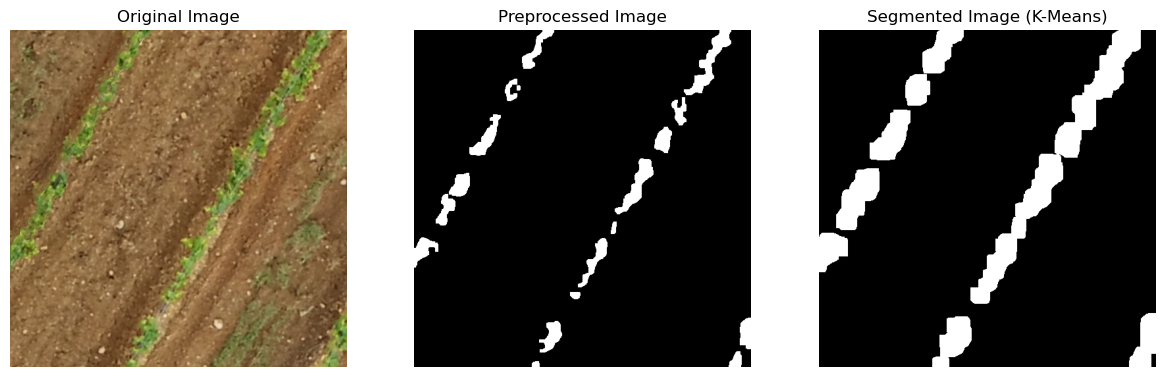
\includegraphics[width=\linewidth]{Kmeans.png}
        \caption{}
        \label{fig2:kmeans}
    \end{subfigure}\hfill
    \begin{subfigure}[b]{0.45\textwidth}
        \centering
        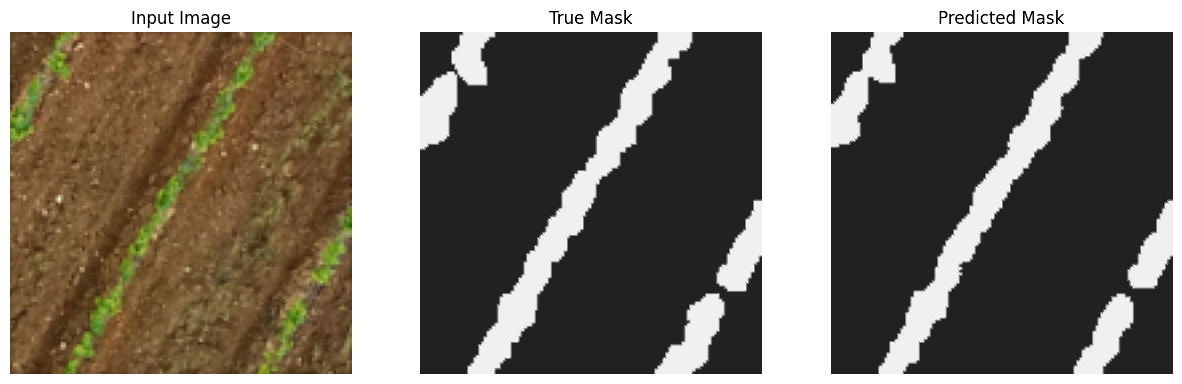
\includegraphics[width=\linewidth]{Dryoutputgrass.png}
        \caption{}
        \label{fig2:filtering}
    \end{subfigure}
    \caption{Crop Detection methods using (a) Color filtering and Kmeans clustering. (b) Unet model}
    \label{fig2:combined}
\end{figure}

\paragraph{Unet-Based Image Segmentation}
The limited performance of color-based image segmentation in crop fields indicates the need for an intelligent model that can recognize the crops using more complicated methods. Utilization of machine learning methods to train semantic segmentation models has proven to be a reliable solution for crop detection. In this approach, a Unet network was chosen as the main image segmentation tool and was trained on a dataset developed by
\cite{b5}
. This dataset consists of UAV-based aerial images taken from three vineyards with corresponding ground truth images, indicating the location of vines in the vineyard.

To use the annotated aerial images, the original and ground truth images were initially split into sub-images, using a sliding window of size 512 by 512 pixels. The step size of sliding was chosen to be 50 pixels, which resulted in more sample data for training. The resulting dataset consists of 5089 sub-images, which are divided into train, test, and validation sets with a ratio of 80\%\
, 10\%\
, 10\%\
.

The Unet model was trained in 50 epochs, which reached the early stopping condition at epoch 7 with an accuracy of 96\%\ and a loss value of 0.09. the predictions of this model on test data prove its ability in semantic segmentation of crops in different conditions, even in the presence of unwanted vegetation. 


\begin{figure}[htbp]
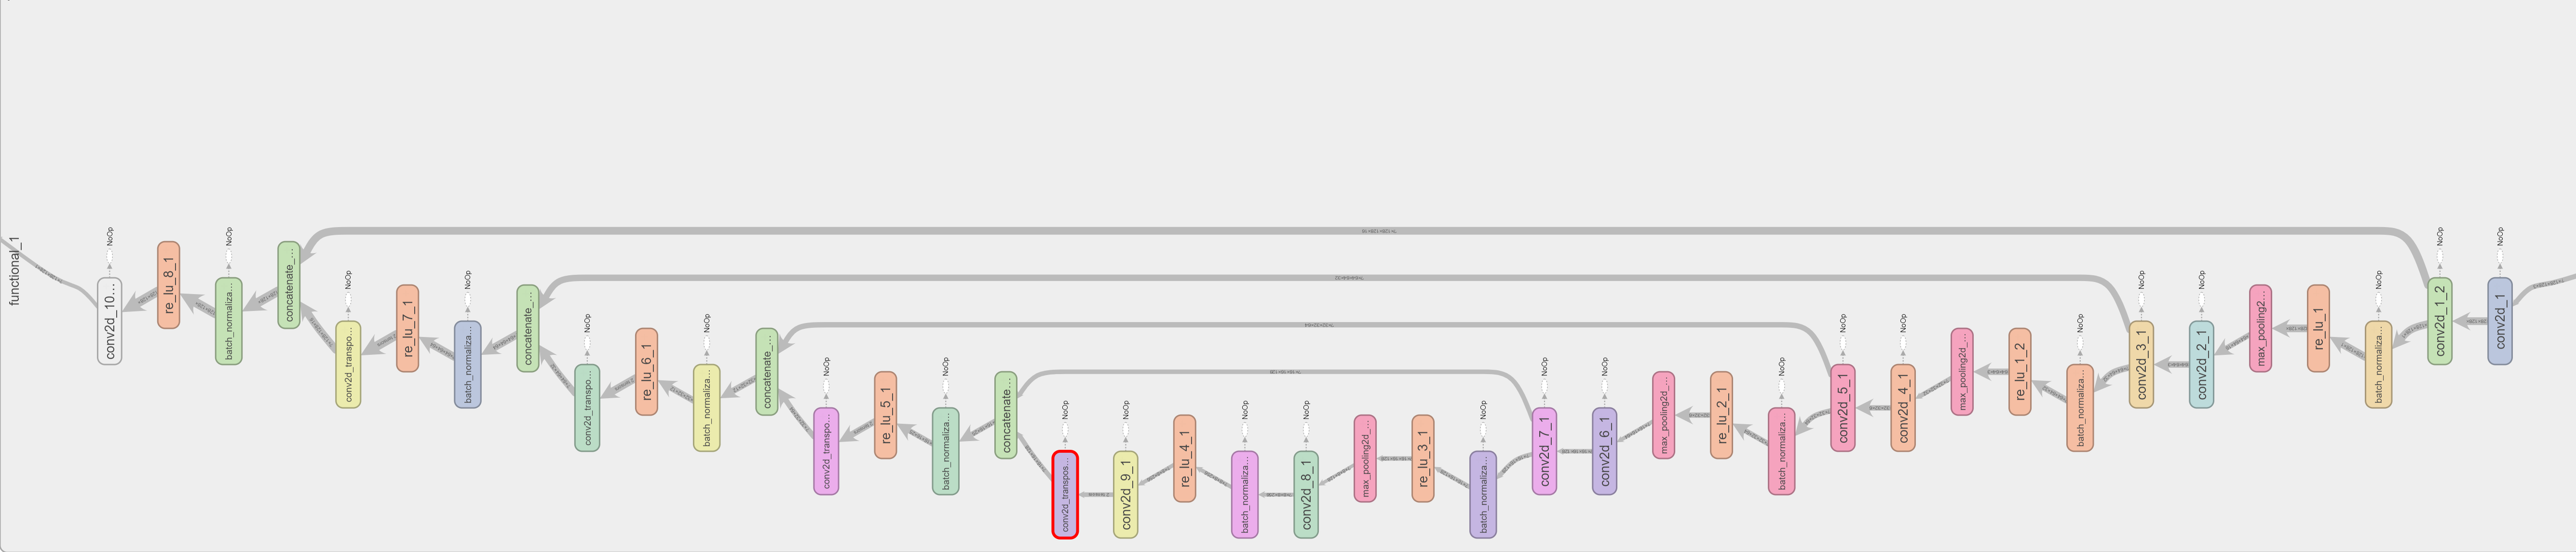
\includegraphics[width=\linewidth]{UNET.png}
\caption{Unet model architecture}
\label{fig3}
\end{figure}

\subsection{Crop Row Detection}\label{Crop Row Detection}
The crop row detection process aims to assign a straight line with a defined slope and intercept to each group of white pixels annotated as crops in the binary mask. This study analyzed and implemented two approaches—linear regression and the Hough Transform—for this purpose.

\subsubsection{Linear Regression}\label{Linear Regression}
This experiment used the binary layer mask of segmented crops to assign each pixel to its corresponding crop row. The first step involved determining the optimal angle of the crop rows through an iterative algorithm, assuming that all rows are parallel and share the same slope. Once the slope was defined, the x and y coordinates of the white pixels were rotated to align the crop rows vertically, simplifying the clustering process.

At this stage, the K-means algorithm was applied with a customized loss function designed to minimize the least square error of the distances between the white pixels and a vertical line. Unlike standard loss functions that measure the distance from a centroid point, this approach considered each cluster centered around a line, not a point.

Given the variability in the number of clusters across different images, the clustering algorithm is initiated by grouping nearby pixels. When a pixel was too distant from the existing group, it was treated as the center of a new cluster. However, this approach led to the formation of numerous unwanted clusters. To address this, adjacent clusters were merged in a subsequent step. Finally, the initial rotation of the pixel coordinates was reversed to visualize the resulting clusters. As illustrated in the results, even after merging close clusters, the method failed to accurately identify crop rows, leading to complications in the later stages of the project. To conclude the experiment, linear regression was applied to fit a line to the pixels within each cluster. However, the results indicated that this clustering and linear regression approach is ineffective for defining crop rows, necessitating exploring alternative methods.

\subsubsection{Hough Transform}\label{Hough Transform}
Another widely used solution for crop row detection is the Hough Transform. This computer vision technique is primarily designed to identify geometric shapes in images, making it particularly effective for detecting lines and curves. In this project, the Hough Transform was employed as an alternative to the linear regression model for predicting crop rows. Implementing this method requires significantly less preprocessing and image manipulation, mainly due to the availability of related packages in OpenCV. When the Hough Transform was applied to the images, multiple lines were detected for each crop row, as illustrated in the results. These lines successfully covered the crop rows, indicating the method's effectiveness in line detection. To refine the results and assign only one line per crop row, the detected lines were merged, and a single line was calculated using the average slope and intercept of the detected lines. The final results are presented in FIGURE.

\begin{figure}[htbp]
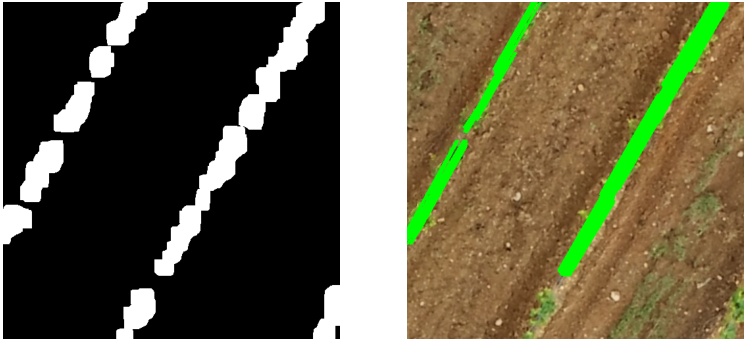
\includegraphics[width=\linewidth]{Hough initial2.png}
\caption{Initial crop row detection using Hough transform}
\label{fig3}
\end{figure}

\subsection{Path Waypoint Detection}\label{Path Waypoint Detection}
As stated in previous steps, the most computational parts of this study are image segmentation and crop row detection. The determination of crop rows as lines with defined slope and intercept makes it straightforward to calculate a line indicating the path. The path is defined as a line parallel to two neighboring crop rows at an equal distance from each. 
Waypoints can be defined by choosing a specific number of equally spaced points along each path. The local coordination of these waypoints is stored to be used in the later steps of the study. 



\begin{figure}[htbp]
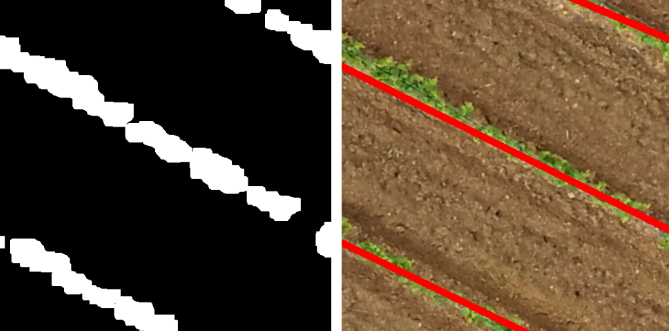
\includegraphics[width=\linewidth]{Hough Revised2.png}
\caption{Modified crop row detection using Hough transform}
\label{fig4}
\end{figure}


\subsection{Reconstruction of Aerial Image}\label{Reconstruction of Aerial Image}
Following the image splitting described in section B.1, the image processing tasks outlined earlier will be applied to each segment of the leading aerial image. The goal is to determine and record the waypoint coordinates within each segment. Once the waypoint coordinates are computed, the initial image must be reconstructed and assembled. Subsequently, the waypoint coordinates need to be converted to align with the coordinates of the newly assembled image.

\section{Image Coordination to Global Coordination Conversion}
An analytical approach and mathematical algorithm are required to obtain the corresponding global coordinates of the points identified in the images. This process involves using the global coordinates of the camera at the time of image capture, along with the camera's height. The conversion process is broken down into two phases: first, converting pixel coordinates into meter distances, and second, converting these meter distances into the global coordinate system.

\subsection{Pixel to Meter Conversion}\label{Pixel to Meter Conversion}
Assuming the camera is positioned at the center of the image at a height of \( h \), and given the angle \( \theta \) (defined as the angle between the standard line from the camera to the ground and the line connecting the camera to the edge of the image), the conversion from pixel position to ground distance is described by the following equations:
\[
\tan \theta = \frac{x}{h} \implies x = \tan \theta  \cdot h
\]
where \( x \) is the distance from the camera to the edge of the image in meters.

If the image length in pixels is denoted as \( L \), then:
\[
1 \text{ pixel} = 2h \cdot \frac{\tan \theta}{L} \text{ (m)}
\]

Using these equations, the position of a pixel with coordinates \((x, y)\) in the image can be determined relative to the camera's position on the ground.

\subsection{Meter to Global Coordination Conversion}\label{Meter to Global Coordination Conversion}
The final step involves converting the meter distances obtained from the previous calculations into global coordinates. The relationship between meters and degrees of latitude or longitude is given by:
\[
1 \text{ (m)} = 0.00001^\circ
\]

This conversion factor enables the translation of local pixel positions, measured in meters, into global coordinates.

\section{Conclusion}\label{Conclusion}
In response to the increasing demand for autonomous agricultural systems, there is a critical need for accurate and reliable waypoints for navigation. This paper presents a solution involving a comprehensive live image capturing, processing, and waypoint generation system. The system is divided into three main sections: data acquisition, which captures and transmits aerial images; image processing, which identifies crops, determines crop rows, and assigns waypoints; and global coordinate conversion, which translates local waypoint coordinates into global coordinates. This approach ensures that the waypoints are precise and suitable for use by mobile robots or other devices requiring accurate navigation within agricultural fields.


\begin{thebibliography}{00}
\bibitem{b1} Y. Yang et al., "Real-time detection of crop rows in maize fields based on autonomous extraction of ROI," Expert Systems with Applications, vol. 213, p. 118826, 2023.
\bibitem{b2} J. Shi, Y. Bai, Z. Diao, J. Zhou, X. Yao, and B. Zhang, "Row detection BASED navigation and guidance for agricultural robots and autonomous vehicles in row-crop fields: methods and applications," Agronomy, vol. 13, no. 7, p. 1780, 2023.
\bibitem{b3} V. R. Ponnambalam, M. Bakken, R. J. Moore, J. Glenn Omholt Gjevestad, and P. Johan From, "Autonomous crop row guidance using adaptive multi-roi in strawberry fields," Sensors, vol. 20, no. 18, p. 5249, 2020.
\bibitem{b4} N. Cunha, T. Barros, M. Reis, T. Marta, C. Premebida, and U. J. Nunes, "Multispectral image segmentation in agriculture: A comprehensive study on fusion approaches," in Iberian Robotics conference, 2023: Springer, pp. 311-323. 
\bibitem{b5} T. Barros et al., "Multispectral vineyard segmentation: A deep learning comparison study," Computers and electronics in agriculture, vol. 195, p. 106782, 2022.
\bibitem{b6} G. Ronchetti, A. Mayer, A. Facchi, B. Ortuani, and G. Sona, "Crop row detection through UAV surveys to optimize on-farm irrigation management," Remote Sensing, vol. 12, no. 12, p. 1967, 2020.
\bibitem{b7} M. Hassanein, M. Khedr, and N. El-Sheimy, "Crop row detection procedure using low-cost UAV imagery system," The International Archives of the Photogrammetry, Remote Sensing and Spatial Information Sciences, vol. 42, pp. 349-356, 2019.
\bibitem{b8} M. D. Bah, A. Hafiane, and R. Canals, "CRowNet: Deep network for crop row detection in UAV images," IEEE Access, vol. 8, pp. 5189-5200, 2019.
\bibitem{b9} I. Sa et al., "WeedMap: A large-scale semantic weed mapping framework using aerial multispectral imaging and deep neural network for precision farming," Remote Sensing, vol. 10, no. 9, p. 1423, 2018.
\bibitem{b10} S. Sankaran et al., "Low-altitude, high-resolution aerial imaging systems for row and field crop phenotyping: A review," European Journal of Agronomy, vol. 70, pp. 112-123, 2015.
\bibitem{b11} L. Comba, P. Gay, J. Primicerio, and D. R. Aimonino, "Vineyard detection from unmanned aerial systems images," Computers and Electronics in Agriculture, vol. 114, pp. 78-87, 2015.
\bibitem{b12} K. Ramesh, N. Chandrika, S. Omkar, M. Meenavathi, and V. Rekha, "Detection of rows in agricultural crop images acquired by remote sensing from a UAV," International Journal of Image, Graphics and Signal Processing, vol. 8, no. 11, p. 25, 2016.
\bibitem{b13} M. Pérez-Ortiz, J. Peña, P. A. Gutiérrez, J. Torres-Sánchez, C. Hervás-Martínez, and F. López-Granados, "A semi-supervised system for weed mapping in sunflower crops using unmanned aerial vehicles and a crop row detection method," Applied Soft Computing, vol. 37, pp. 533-544, 2015.
\bibitem{b14} Y. Pang et al., "Improved crop row detection with deep neural network for early-season maize stand count in UAV imagery," Computers and Electronics in Agriculture, vol. 178, p. 105766, 2020.
\bibitem{b15} N. Samet, S. Hicsonmez, and E. Akbas, "Houghnet: Integrating near and long-range evidence for bottom-up object detection," in Computer Vision–ECCV 2020: 16th European Conference, Glasgow, UK, August 23–28, 2020, Proceedings, Part XXV 16, 2020: Springer, pp. 406-423. 
\end{thebibliography}

\vspace{12pt}


\end{document}
